% Options for packages loaded elsewhere
\PassOptionsToPackage{unicode}{hyperref}
\PassOptionsToPackage{hyphens}{url}
\PassOptionsToPackage{dvipsnames,svgnames,x11names}{xcolor}
%
\documentclass[
  letterpaper,
  DIV=11,
  numbers=noendperiod]{scrartcl}

\usepackage{amsmath,amssymb}
\usepackage{lmodern}
\usepackage{iftex}
\ifPDFTeX
  \usepackage[T1]{fontenc}
  \usepackage[utf8]{inputenc}
  \usepackage{textcomp} % provide euro and other symbols
\else % if luatex or xetex
  \usepackage{unicode-math}
  \defaultfontfeatures{Scale=MatchLowercase}
  \defaultfontfeatures[\rmfamily]{Ligatures=TeX,Scale=1}
\fi
% Use upquote if available, for straight quotes in verbatim environments
\IfFileExists{upquote.sty}{\usepackage{upquote}}{}
\IfFileExists{microtype.sty}{% use microtype if available
  \usepackage[]{microtype}
  \UseMicrotypeSet[protrusion]{basicmath} % disable protrusion for tt fonts
}{}
\makeatletter
\@ifundefined{KOMAClassName}{% if non-KOMA class
  \IfFileExists{parskip.sty}{%
    \usepackage{parskip}
  }{% else
    \setlength{\parindent}{0pt}
    \setlength{\parskip}{6pt plus 2pt minus 1pt}}
}{% if KOMA class
  \KOMAoptions{parskip=half}}
\makeatother
\usepackage{xcolor}
\setlength{\emergencystretch}{3em} % prevent overfull lines
\setcounter{secnumdepth}{-\maxdimen} % remove section numbering
% Make \paragraph and \subparagraph free-standing
\ifx\paragraph\undefined\else
  \let\oldparagraph\paragraph
  \renewcommand{\paragraph}[1]{\oldparagraph{#1}\mbox{}}
\fi
\ifx\subparagraph\undefined\else
  \let\oldsubparagraph\subparagraph
  \renewcommand{\subparagraph}[1]{\oldsubparagraph{#1}\mbox{}}
\fi


\providecommand{\tightlist}{%
  \setlength{\itemsep}{0pt}\setlength{\parskip}{0pt}}\usepackage{longtable,booktabs,array}
\usepackage{calc} % for calculating minipage widths
% Correct order of tables after \paragraph or \subparagraph
\usepackage{etoolbox}
\makeatletter
\patchcmd\longtable{\par}{\if@noskipsec\mbox{}\fi\par}{}{}
\makeatother
% Allow footnotes in longtable head/foot
\IfFileExists{footnotehyper.sty}{\usepackage{footnotehyper}}{\usepackage{footnote}}
\makesavenoteenv{longtable}
\usepackage{graphicx}
\makeatletter
\def\maxwidth{\ifdim\Gin@nat@width>\linewidth\linewidth\else\Gin@nat@width\fi}
\def\maxheight{\ifdim\Gin@nat@height>\textheight\textheight\else\Gin@nat@height\fi}
\makeatother
% Scale images if necessary, so that they will not overflow the page
% margins by default, and it is still possible to overwrite the defaults
% using explicit options in \includegraphics[width, height, ...]{}
\setkeys{Gin}{width=\maxwidth,height=\maxheight,keepaspectratio}
% Set default figure placement to htbp
\makeatletter
\def\fps@figure{htbp}
\makeatother

\usepackage{booktabs}
\usepackage{longtable}
\usepackage{array}
\usepackage{multirow}
\usepackage{wrapfig}
\usepackage{float}
\usepackage{colortbl}
\usepackage{pdflscape}
\usepackage{tabu}
\usepackage{threeparttable}
\usepackage{threeparttablex}
\usepackage[normalem]{ulem}
\usepackage{makecell}
\usepackage{xcolor}
\KOMAoption{captions}{tableheading}
\makeatletter
\makeatother
\makeatletter
\makeatother
\makeatletter
\@ifpackageloaded{caption}{}{\usepackage{caption}}
\AtBeginDocument{%
\ifdefined\contentsname
  \renewcommand*\contentsname{Table of contents}
\else
  \newcommand\contentsname{Table of contents}
\fi
\ifdefined\listfigurename
  \renewcommand*\listfigurename{List of Figures}
\else
  \newcommand\listfigurename{List of Figures}
\fi
\ifdefined\listtablename
  \renewcommand*\listtablename{List of Tables}
\else
  \newcommand\listtablename{List of Tables}
\fi
\ifdefined\figurename
  \renewcommand*\figurename{Figure}
\else
  \newcommand\figurename{Figure}
\fi
\ifdefined\tablename
  \renewcommand*\tablename{Table}
\else
  \newcommand\tablename{Table}
\fi
}
\@ifpackageloaded{float}{}{\usepackage{float}}
\floatstyle{ruled}
\@ifundefined{c@chapter}{\newfloat{codelisting}{h}{lop}}{\newfloat{codelisting}{h}{lop}[chapter]}
\floatname{codelisting}{Listing}
\newcommand*\listoflistings{\listof{codelisting}{List of Listings}}
\makeatother
\makeatletter
\@ifpackageloaded{caption}{}{\usepackage{caption}}
\@ifpackageloaded{subcaption}{}{\usepackage{subcaption}}
\makeatother
\makeatletter
\@ifpackageloaded{tcolorbox}{}{\usepackage[many]{tcolorbox}}
\makeatother
\makeatletter
\@ifundefined{shadecolor}{\definecolor{shadecolor}{rgb}{.97, .97, .97}}
\makeatother
\makeatletter
\makeatother
\ifLuaTeX
  \usepackage{selnolig}  % disable illegal ligatures
\fi
\IfFileExists{bookmark.sty}{\usepackage{bookmark}}{\usepackage{hyperref}}
\IfFileExists{xurl.sty}{\usepackage{xurl}}{} % add URL line breaks if available
\urlstyle{same} % disable monospaced font for URLs
\hypersetup{
  pdftitle={Agriculture Total Factor Production in Global Income Classes},
  pdfauthor={Gabrielle Smith},
  colorlinks=true,
  linkcolor={blue},
  filecolor={Maroon},
  citecolor={Blue},
  urlcolor={Blue},
  pdfcreator={LaTeX via pandoc}}

\title{Agriculture Total Factor Production in Global Income Classes}
\author{Gabrielle Smith}
\date{2022-12-03}

\begin{document}
\maketitle
\ifdefined\Shaded\renewenvironment{Shaded}{\begin{tcolorbox}[borderline west={3pt}{0pt}{shadecolor}, sharp corners, boxrule=0pt, interior hidden, enhanced, frame hidden, breakable]}{\end{tcolorbox}}\fi

\renewcommand*\contentsname{Table of contents}
{
\hypersetup{linkcolor=}
\setcounter{tocdepth}{3}
\tableofcontents
}
\hypertarget{introduction}{%
\subsubsection{Introduction}\label{introduction}}

The agricultural sector faces opposing pressures of sustaining a growing
population while minimizing its unfavorable outcomes on finite
environmental resources\footnote{Network on Agricultural Total Factor
  Productivity and the Environment. Oecd.org. Accessed December 4, 2022.
  https://www.oecd.org/agriculture/topics/network-agricultural-productivity-and-environment/}.
In an effort to simultaneously move towards these goals, countries
around the world have prioritized agricultural productivity. One of the
most informative measures of agricultural productivity is total factor
productivity (TFP). TFP compares gross outputs of crop, animal and
aquaculture products to inputs of land, labor, capital and material
resources utilized in farm production\footnote{Fuglie K, Jelliffe J,
  Morgan S. Documentation and methods. Usda.gov. Published October 7,
  2022. Accessed December 4, 2022.
  https://www.ers.usda.gov/data-products/international-agricultural-productivity/documentation-and-methods/}.
As gross output increases at a faster rate than total inputs, total
factor production improves, which eases tensions on environmental
resources and food security, and boosts economic growth\footnote{Fuglie
  K, Jelliffe J, Morgan S. Documentation and methods. Usda.gov.
  Published October 7, 2022. Accessed December 4, 2022.
  https://www.ers.usda.gov/data-products/international-agricultural-productivity/documentation-and-methods/}.
TFP is expressed generally by the equation:

\[TFP = Y/X\]

where Y represents gross output and X represents total inputs.

TFP is an important measure for informing policy priorities for
agricultural productivity. These policies include investments in
research and development, incentivizing economic reforms for farmers,
rural education and extension, and improvments in
infrastructure\footnote{Fuglie K, Wang SL. New Evidence Points to Robust
  But Uneven Productivity Growth in Global Agriculture. Usda.gov.
  Published September 20, 2012. Accessed December 4, 2022.
  https://www.ers.usda.gov/amber-waves/2012/september/global-agriculture/}.
Understanding the effects of individual inputs on TFP can direct
decision making as it relates to resource allocation for these policy
investments.

\begin{figure}

{\centering 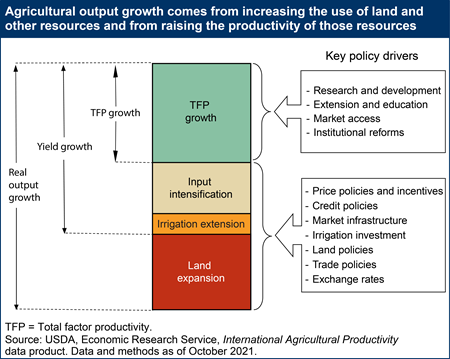
\includegraphics{usda_output.png}

}

\end{figure}

This analysis will regress global TFP indices on inputs of land, labor,
capital, and materials to examine the effects of these inputs on gross
outputs. This regression can be utilized to maximize TFP growth rates by
differentiating efficiency levels of individual inputs as they relate to
gross productivity, which can direct resource allocation to
technological improvements of inefficient input systems.

Additionally, it will examine TFP growth rates for country groupings of
income class (defined by the {[}World
Bank{]}(https://blogs.worldbank.org/opendata/new-world-bank-country-classifications-income-level-2021-2022))
by testing for mean differences. It will also forecast TFP growth rates
for years 2020-2030 at a global scale and for income classes by
employing automated autoregressive moving average (ARIMA) models.
Understanding nuances in TFP growth for varying income scales can be
useful in further research to refine regressions that direct policy
prioritization.

All relevant analysis outputs are included in the Analysis section - for
detailed code concerning model checking, reference the Model Testing and
Supporting Figures section.

\hypertarget{data}{%
\subsubsection{Data}\label{data}}

Data used in this analysis is sourced from the United States Department
of Agriculture's (USDA) Economic Research Services\footnote{Fuglie K,
  Jelliffe J, Morgan S. International agricultural productivity.
  Usda.gov. Published October 7, 2022. Accessed December 4, 2022.
  https://www.ers.usda.gov/data-products/international-agricultural-productivity/}.
This data is publicly available
\href{https://www.ers.usda.gov/data-products/international-agricultural-productivity/}{here}.
Data files contain annual indices for agricultural TFP, outputs, and
inputs for individual countries, major global regions, and countries
grouped by income levels for years 1961-2020. Detailed data on land,
labor, capital and material inputs used to construct TFP indices is also
included, but are not contained in the subsetted data used for the
purposes of this particular analysis. TFPs are indexed with a base year
of 2015 such that TFP values for countries and regions are set to 100 in
2015.

It is relevant to note that TFP index comparison between geographical
regions provides information regarding TFP growth rates, but is not
informative for direct comparison of productivity levels.

\hypertarget{analysis}{%
\subsubsection{Analysis}\label{analysis}}

\hypertarget{multiple-linear-regression}{%
\paragraph{Multiple Linear
Regression}\label{multiple-linear-regression}}

A stepwise regression is performed to compare a linear model containing
no predictors to a full linear model containing all input variables
(land, labor, capital, and materials). The results of this regression
suggest that materials are not a relevant predictor in estimating TFP.
Consequently, we opt for a model containing three predictor variables:
land, labor, capital.

Full model:
\[TFP = \beta_0 + \beta_1*land_i + \beta_2*labor_i + \beta_3*capital_i + \beta_4 * materials_i + \varepsilon_i\]

Reduced model:
\[TFP = \beta_0 + \beta_1*land_i + \beta_2*labor_i + \beta_3*capital_i  + \varepsilon_i\]

The r-squared, adjusted r-squared, and Mallow's Cp values of the leaps
procedure affirm that this model is optimal in predictive accuracy. A
pairwise analysis of the reduced predictor variables suggests that there
may be significant variable interactions. A second stepwise regression
is performed with a full linear model containing all interactions
between refined predictor variables, which suggests that there is a
significant interaction between land and capital inputs. Therefore, we
include this interaction term in the refined model.

Full model:
\[TFP = \beta_0 + \beta_1*land_i + \beta_2*labor_i + \beta_3*capital_i  + \beta_4*land_i:capital_i + \\ \beta_5*land_i:labor_i + \beta_6*land_i:capital_i + \varepsilon_i\]

Reduced model:
\[TFP = \beta_0 + \beta_1*land_i + \beta_2*labor_i + \beta_3*capital_i + \beta_4 * land_i:capital_i + \varepsilon_i\]

The Normal Q-Q plot of the residuals evidences slight non-normality. A
log transformation of the response variable, TFP, is performed for
normalization.

A summary of the updated model is evaluated. A Residuals vs.~Fitted plot
displays a roughly even spread of residuals around the zero line, which
suggests that equal variance and linearity assumptions are satisfied. A
Normal Q-Q plot suggests normality given its relative linearity.
Therefore, we accept the reduced and transformed model as a final model.

Accepted model:
\[log(TFP) = \beta_0 + \beta_1*land_i + \beta_2*labor_i + \beta_3*capital_i + \beta_4 * land_i:capital_i + \varepsilon_i\]

\begin{longtable}[]{@{}cccc@{}}
\caption{Tbl 1. Transformed Linear Model Results for TFP
Regression}\tabularnewline
\toprule()
~ &
\multicolumn{3}{>{\centering\arraybackslash}p{(\columnwidth - 6\tabcolsep) * \real{0.0000} + 4\tabcolsep}@{}}{%
Log Total Factor Production} \\
\midrule()
\endfirsthead
\toprule()
~ &
\multicolumn{3}{>{\centering\arraybackslash}p{(\columnwidth - 6\tabcolsep) * \real{0.0000} + 4\tabcolsep}@{}}{%
Log Total Factor Production} \\
\midrule()
\endhead
Predictors & Estimates & 95\% Conf. Interval & P-value \\
Intercept & 4.5154529 & 4.4889663~--~4.5419395 &
\textbf{\textless0.001} \\
Land & 0.0008662 & 0.0005873~--~0.0011451 & \textbf{\textless0.001} \\
Labor & -0.0019178 & -0.0021221~--~-0.0017135 &
\textbf{\textless0.001} \\
Capital & -0.0000779 & -0.0001752~--~0.0000194 & 0.117 \\
Land * Capital & 0.0000062 & 0.0000047~--~0.0000077 &
\textbf{\textless0.001} \\
Observations &
\multicolumn{3}{>{\raggedright\arraybackslash}p{(\columnwidth - 6\tabcolsep) * \real{0.0000} + 4\tabcolsep}@{}}{%
10187} \\
R\textsuperscript{2} / R\textsuperscript{2} adjusted &
\multicolumn{3}{>{\raggedright\arraybackslash}p{(\columnwidth - 6\tabcolsep) * \real{0.0000} + 4\tabcolsep}@{}}{%
0.075 / 0.075} \\
\bottomrule()
\end{longtable}

Given coefficient estimates of our performed regression, the final model
is represented as:

\[log(TFP) = 4.515429 + 0.0008662*land_i - 0.0019178*labor_i - 0.0000779*capital_i + \\ 0.0000062 * land_i:capital_i + \varepsilon_i\]

The model regression indicates that capital is not a significant
predictor variable (p = 0.117); however, all other predictor variables
are found to be significant at the 0.001 level (p \textless{} 0.001 for
all remaining variables). Given that the interaction between land and
capital variables is significant (p \textless{} 0.001), we opt to
preserve capital as a predictor variable in spite of its insignificant
predictive power. It is relevant to note that the model summary values
are based off of a log-transformed model - for interpretability of these
results, it is recommended an inverse transformation be performed on the
model estimates. In spite of this, given the signs of the estimates, it
can be noted that labor and capital inputs are negatively correlated
with TFP, while land and land/capital interaction inputs are positively
correlated with TFP. The overall predictive power of the model is low
(evidenced by adjusted r-squared = 0.075), which suggests that it is not
well equipped to accurately predict TFP variability.

\hypertarget{differences-in-means-for-varying-world-economies}{%
\paragraph{Differences in Means for Varying World
Economies}\label{differences-in-means-for-varying-world-economies}}

We move to performing statistical tests to compare means of TFP indices
between countries grouped by income class: low income (LI), lower-middle
income (MI-L), upper-middle income (MI-U), high income (HI). Our first
step is to visualize the distribution of the data for all income
classes.

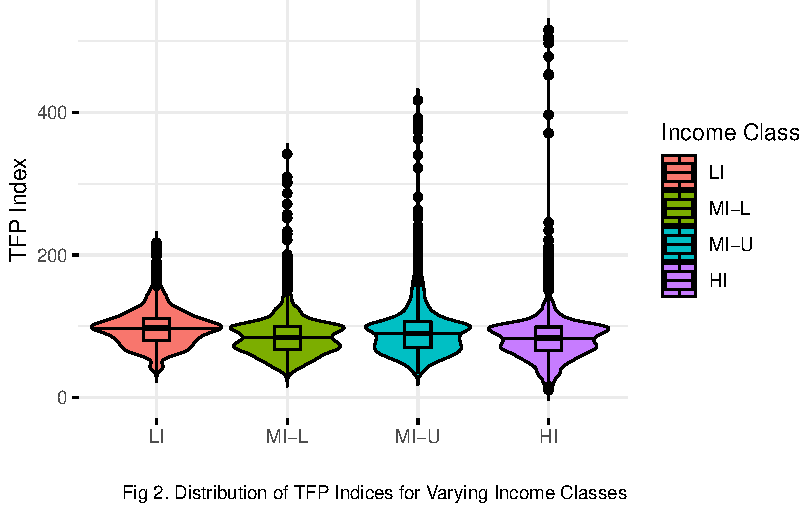
\includegraphics{Smith_Gabrielle_EDS222Final_files/figure-pdf/unnamed-chunk-4-1.pdf}

Given that there are significant outliers in each income class, mean
differences are tested using Kruskal-Wallis and Dunn tests, both
non-parametric methods that have no assumptions of normality.

The null hypothesis:
\[H_0: \mu_{low}=\mu_{mid-low} = \mu_{mid-high} = \mu_{high}\]

The alternative hypothesis:

H\textsubscript{A}: mean TFP indices are not equal across all income
classes

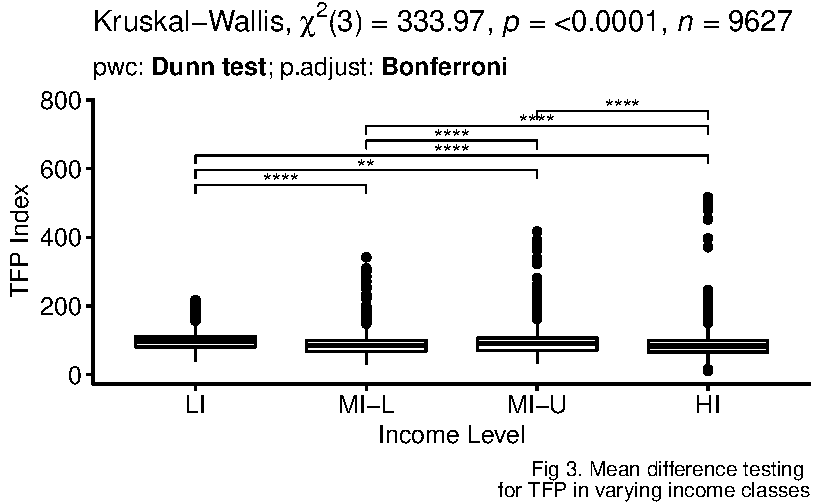
\includegraphics{Smith_Gabrielle_EDS222Final_files/figure-pdf/unnamed-chunk-5-1.pdf}

The Kruskal-Wallis test (p\textless0.0001) rejects the null hypothesis;
there is significant evidence to suggest that there is a difference in
mean TFP indices between differing income classes. The Dunn test
concludes that this difference is statistically significant between all
income class pairings, indicated by significance asterisks of the above.
We use this information primarily to validate the productivity of
forecasting TFP growth at income class scales as opposed to globally,
rather than for the purpose of directly comparing mean differences,
since dataset indexing invalidates the capacity for direct productivity
comparisons between groups.

\hypertarget{tfp-growth-forecasting}{%
\paragraph{TFP Growth Forecasting}\label{tfp-growth-forecasting}}

We employ autoregressive integrated moving average (ARIMA) models to
predict global and income class grouped TFP indices until year 2030.

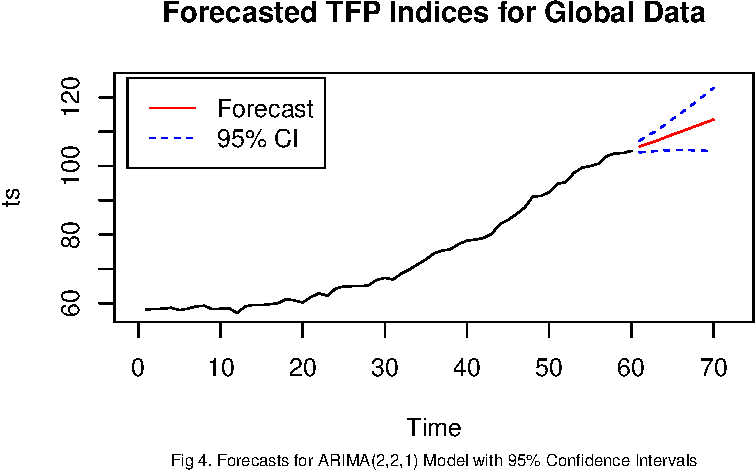
\includegraphics{Smith_Gabrielle_EDS222Final_files/figure-pdf/unnamed-chunk-6-1.pdf}

Based on historical trend, the forecast anticipates that global TFP will
continue to grow in the coming decade. We look to forecasted values for
more detailed information concerning this growth.

\begin{table}

\caption{Tbl 2. Predicted TFP Indices}
\centering
\begin{tabular}[t]{r|r|r|r|r|r}
\hline
Year & Low Income & Lower-Middle Income & Upper-Middle Income & High Income & World\\
\hline
2021 & 101.8986 & 103.8871 & 102.379 & 105.5007 & 105.6913\\
\hline
2022 & 101.8986 & 104.3529 & 102.379 & 106.4207 & 106.5413\\
\hline
2023 & 101.8986 & 104.9014 & 102.379 & 107.3407 & 107.2756\\
\hline
2024 & 101.8986 & 105.5635 & 102.379 & 108.2607 & 108.2272\\
\hline
2025 & 101.8986 & 106.1743 & 102.379 & 109.1807 & 109.1500\\
\hline
2026 & 101.8986 & 106.7559 & 102.379 & 110.1007 & 109.9950\\
\hline
2027 & 101.8986 & 107.3610 & 102.379 & 111.0207 & 110.8787\\
\hline
2028 & 101.8986 & 107.9716 & 102.379 & 111.9407 & 111.7803\\
\hline
2029 & 101.8986 & 108.5730 & 102.379 & 112.8607 & 112.6601\\
\hline
2030 & 101.8986 & 109.1743 & 102.379 & 113.7807 & 113.5402\\
\hline
\end{tabular}
\end{table}

The automated models for income class groups predict that low income and
upper-middle income class countries will see no change in TFP indices
throughout the forecasted decade. The models also predict that
lower-middle income and high income countries will experience steady
growth in TFP indices, which is reflected similarly in predicted
consistent TFP growth for non-grouped world data.

\hypertarget{discussion}{%
\subsubsection{Discussion}\label{discussion}}

The maximization of agricultural total factor productivity will promote
sustainable economic growth and can be used as a tool to ease the
environmental burden of agriculture, so understanding the effects of
inputs in TFP is pertinent to resource allocation in policy drivers.

Results of the linear regression evidence that only land, labor, and
land/capital interaction inputs are significant predictors of TFP,
although we preserve capital inputs in our model due to its significance
in interaction terms. The global model's coefficient estimates indicate
that land and land/capital interaction inputs are positively correlated
with TFP - that is, growth rates of these inputs correlate to
comparatively larger growth rates of gross outputs. Inversely, labor and
capital inputs are negatively correlated with TFP - while increased
inputs of these variables may increase total outputs, the growth rate of
associated outputs is smaller than than the growth rate of its inputs.

For quantitative interpretations, we would transform summary
coefficients following the equation
\[(\exp(coefficient.estimate)-1)*100\] such that they reflect percent
increases (as opposed to unit increases) of the response variable, TFP,
for one-unit increases in associated input variables.

Mean testing indicates that there is a statistically significant
difference in mean TFP values between all income class pairs. A
one-sided test of means may offer more insight regarding income class
TFP distinctions.

The time series forecasting of TFP indices exhibits predicted increases
in global TFP indices in the next decade, yet only lower-middle income
and high income classifications are expected to see growing TFP, while
low income and upper-middle income classifications are predicted to
stagnate. As it pertains to low-income countries, it is reasonable to
assume that there is limited flexibility for expenditure on the research
and development that TFP growth necessitates, so this stagnation is
largely unsurprising. A potential explanation for upper-middle income
TFP stagnation is the
\href{https://elibrary.worldbank.org/doi/10.1596/9780821387856_CH04}{``middle-income
trap''}\footnote{Griffith B. Middle-Income Trap. In: Frontiers in
  Development Policy. The World Bank; 2011:39-43.}. However, these
theories are largely assumptive. Cross-country differences in TFP growth
within income classes is highly variable and depend on numerous factors
including research and development, enabling environments, and
economically disruptive shocks\footnote{Fuglie K, Wang SL. New Evidence
  Points to Robust But Uneven Productivity Growth in Global Agriculture.
  Usda.gov. Published September 20, 2012. Accessed December 4, 2022.
  https://www.ers.usda.gov/amber-waves/2012/september/global-agriculture/},
so forecasting measures are expected to be more informative and accurate
for predictive models fit to a particular country of interest.

\hypertarget{further-research}{%
\subsubsection{Further Research}\label{further-research}}

Under the produced linear model, only 7.5\% of variation in global TFP
is explained by the model's input variables (Tbl 1). It is reasonable to
expect that a global model utilizing detailed land, labor, capital, and
materials variables may perform better than a model comprised of only
their summative indexes. A best fitting model to inform policy
prioritization will be tailored to a particular country of interest,
which eliminates the variability of cross-country differences in TFP.

Furthermore, some of the residuals of the automated predictive models
appear to be significant beyond the randomness of white noise (see Model
Checking and Supporting Figures), which implies potential to produce
more accurate forecasting models for income class groupings.

Finally, current measures of TFP do not factor environmental impacts.
Growing productivity rates ease natural resource demand in agriculture,
which lessens pressure on finite environmental reserves; however, higher
productivity can also result in higher externalities that negatively
impact the environment. The
\href{https://www.oecd.org/agriculture/topics/network-agricultural-productivity-and-environment/}{Network
on Agricultural TFP and the Environment}, launched in 2017, aims to
develop a framework for cross-country agricultural TFP comparisons to
help address this issue\footnote{Network on Agricultural Total Factor
  Productivity and the Environment. Oecd.org. Accessed December 4, 2022.
  https://www.oecd.org/agriculture/topics/network-agricultural-productivity-and-environment/}.

\hypertarget{conclusion}{%
\subsubsection{Conclusion}\label{conclusion}}

This analysis lends itself to understanding how policy priorities can be
shaped to maximize agricultural TFP growth through individual inputs,
and examines the differences of this index across various levels of
income class.

\hypertarget{model-testing-and-supporting-figures}{%
\subsubsection{Model Testing and Supporting
Figures}\label{model-testing-and-supporting-figures}}

\begin{verbatim}
  (Intercept)    x1   x2    x3
1        TRUE FALSE TRUE FALSE
2        TRUE  TRUE TRUE FALSE
3        TRUE  TRUE TRUE  TRUE
\end{verbatim}

\begin{verbatim}
[1] 0.03808702 0.04533486 0.04966514
\end{verbatim}

\begin{verbatim}
[1] 0.03799258 0.04514738 0.04938516
\end{verbatim}

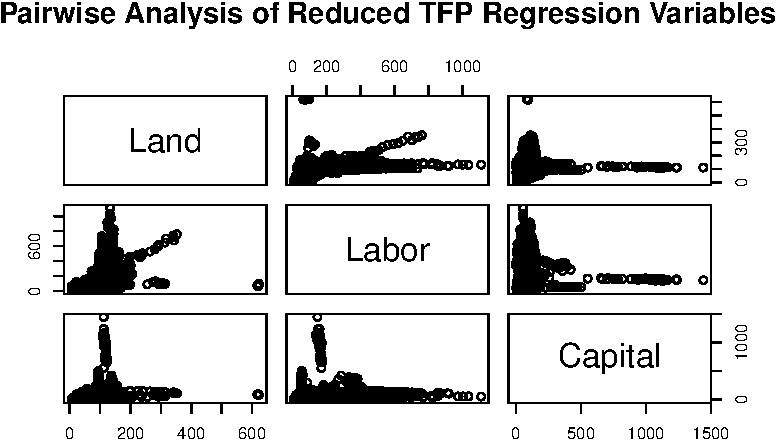
\includegraphics{Smith_Gabrielle_EDS222Final_files/figure-pdf/unnamed-chunk-9-1.pdf}

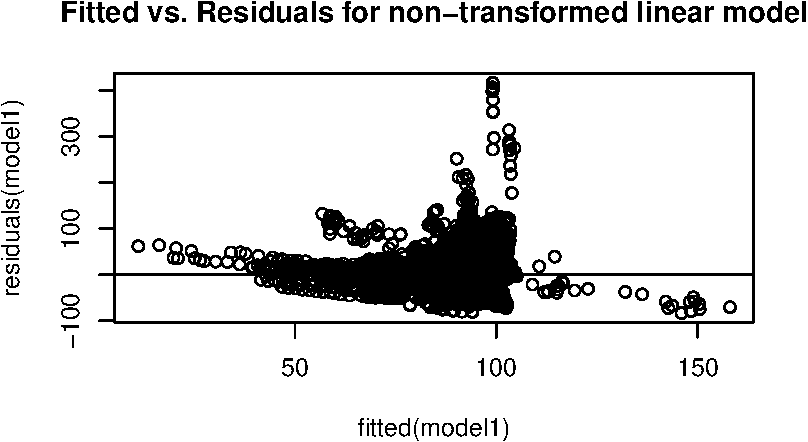
\includegraphics{Smith_Gabrielle_EDS222Final_files/figure-pdf/unnamed-chunk-10-1.pdf}

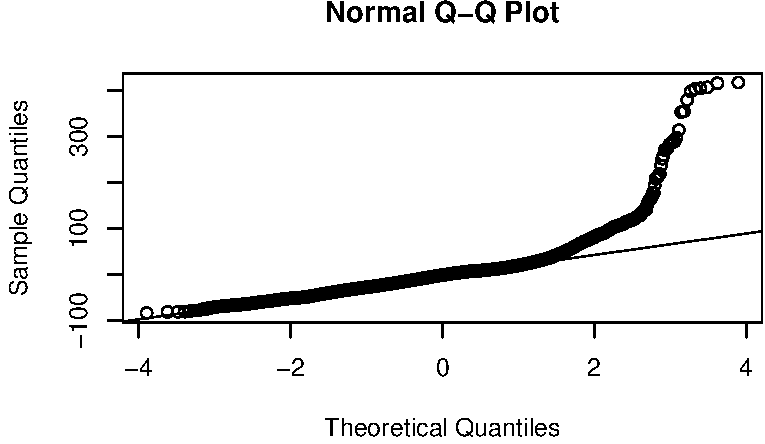
\includegraphics{Smith_Gabrielle_EDS222Final_files/figure-pdf/unnamed-chunk-10-2.pdf}

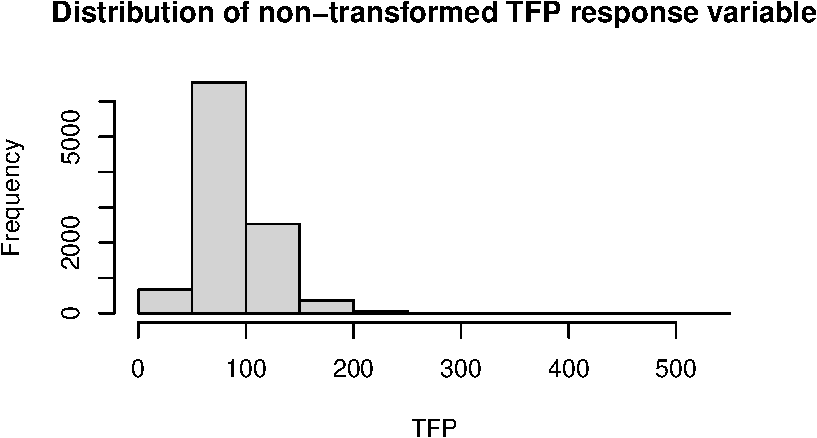
\includegraphics{Smith_Gabrielle_EDS222Final_files/figure-pdf/unnamed-chunk-10-3.pdf}

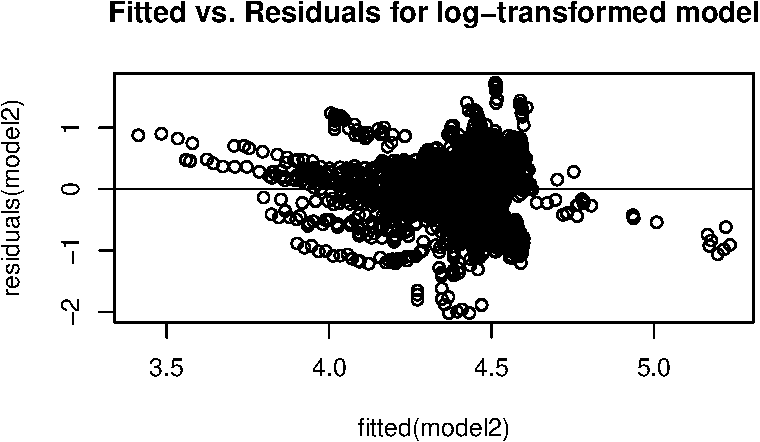
\includegraphics{Smith_Gabrielle_EDS222Final_files/figure-pdf/unnamed-chunk-11-1.pdf}

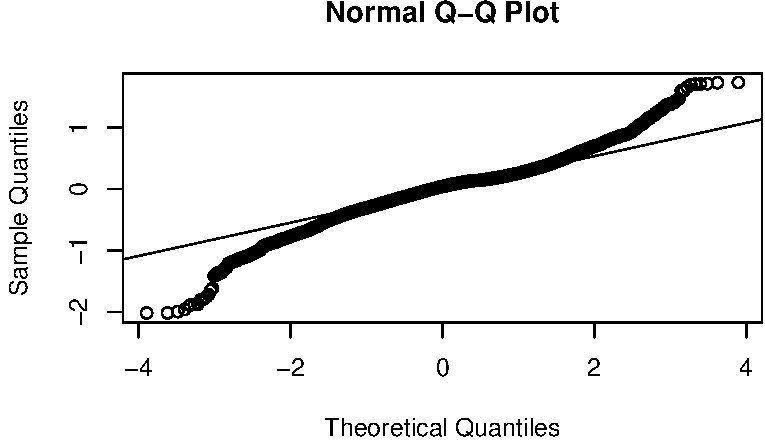
\includegraphics{Smith_Gabrielle_EDS222Final_files/figure-pdf/unnamed-chunk-11-2.pdf}

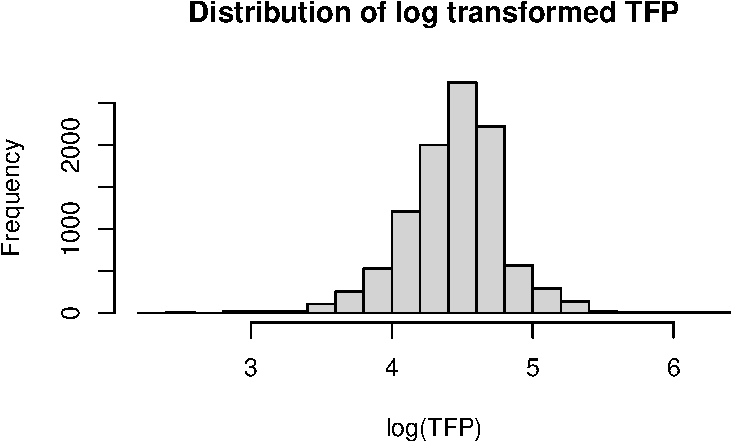
\includegraphics{Smith_Gabrielle_EDS222Final_files/figure-pdf/unnamed-chunk-11-3.pdf}

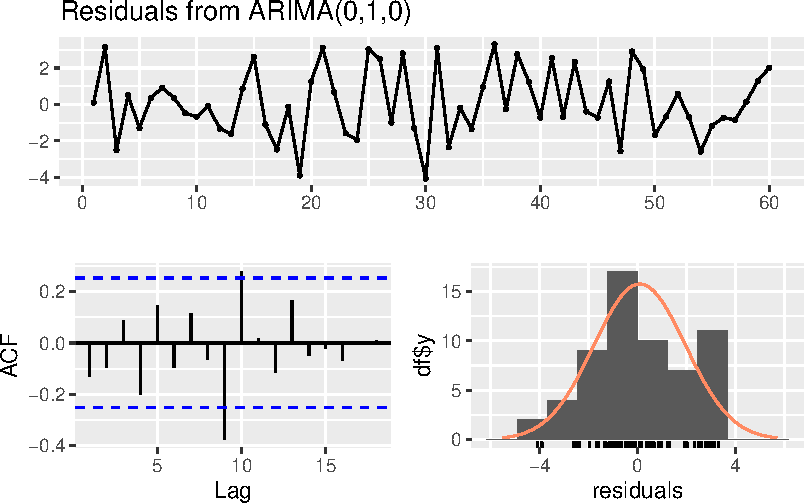
\includegraphics{Smith_Gabrielle_EDS222Final_files/figure-pdf/unnamed-chunk-12-1.pdf}

\begin{verbatim}

    Ljung-Box test

data:  Residuals from ARIMA(0,1,0)
Q* = 24.192, df = 10, p-value = 0.007108

Model df: 0.   Total lags used: 10
\end{verbatim}

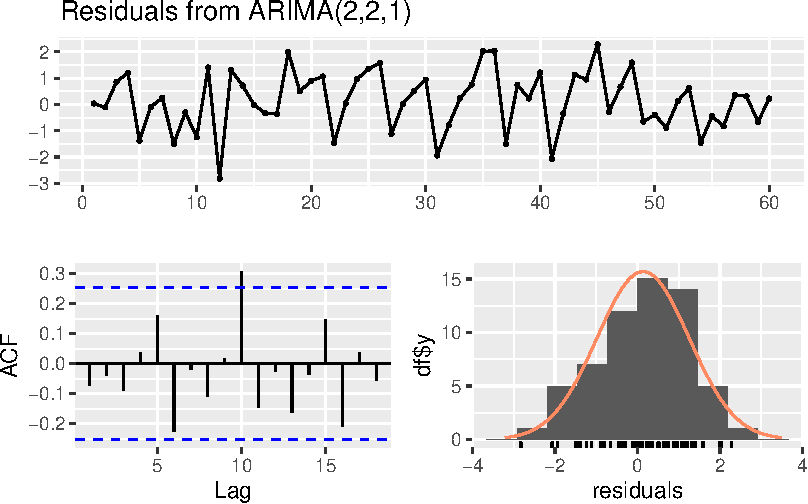
\includegraphics{Smith_Gabrielle_EDS222Final_files/figure-pdf/unnamed-chunk-13-1.pdf}

\begin{verbatim}

    Ljung-Box test

data:  Residuals from ARIMA(2,2,1)
Q* = 14.191, df = 7, p-value = 0.04788

Model df: 3.   Total lags used: 10
\end{verbatim}

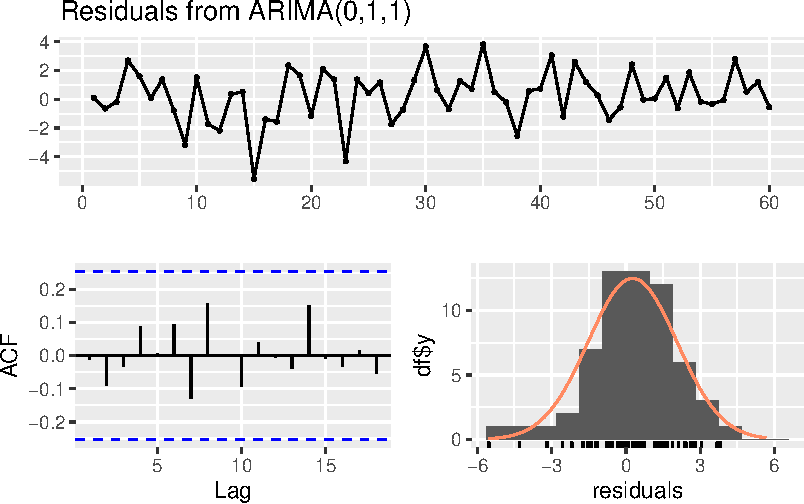
\includegraphics{Smith_Gabrielle_EDS222Final_files/figure-pdf/unnamed-chunk-14-1.pdf}

\begin{verbatim}

    Ljung-Box test

data:  Residuals from ARIMA(0,1,1)
Q* = 5.3068, df = 9, p-value = 0.8068

Model df: 1.   Total lags used: 10
\end{verbatim}

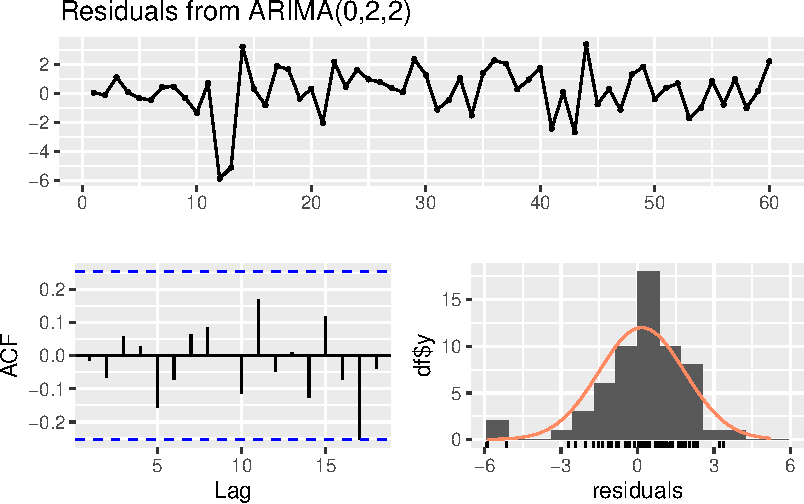
\includegraphics{Smith_Gabrielle_EDS222Final_files/figure-pdf/unnamed-chunk-15-1.pdf}

\begin{verbatim}

    Ljung-Box test

data:  Residuals from ARIMA(0,2,2)
Q* = 4.4176, df = 8, p-value = 0.8176

Model df: 2.   Total lags used: 10
\end{verbatim}



\end{document}
